\section{Results and Discussion}
\label{sec:results}

\subsection{Quantitative Snapshot from Phase 4}

Table~\ref{tab:phase4-results} is updated from the saved outputs of \textit{Phase 4 - Evaluation and Analysis} (Task 4.1). All six models are evaluated on the same 100-sample test split.

\begin{table}[H]
	\centering
	\caption{Phase 4 overall performance summary (Task 4.1).}
	\label{tab:phase4-results}
	\scriptsize
	\setlength{\tabcolsep}{3.5pt}
	\resizebox{\columnwidth}{!}{%
	\begin{tabular}{lcccc}
		\toprule
		Model & Mod. & Epochs & Acc. (\%) & Macro-F1 \\
		\midrule
		N1 (FC) & Img & 100 & 53.0 & 0.5185 \\
		N2 (CNN) & Img & 100 & 61.0 & 0.6019 \\
		N3 (CNN+BN) & Img & 100 & 70.0 & 0.6853 \\
		N4 (CNN+BN+RMSp) & Img & 100 & 67.0 & 0.6621 \\
		N5 (LSTM) & Aud & 50 & 69.0 & 0.6805 \\
		N6 (LSTM+GAN) & Aud & 50 & 71.0 & 0.7045 \\
		\bottomrule
	\end{tabular}%
	}
\end{table}

\begin{table}[t]
	\centering
	\caption{Architecture/optimizer impact from \texttt{phase4\_architecture\_impact.csv}.}
	\label{tab:phase4-impact}
	\scriptsize
	\setlength{\tabcolsep}{4pt}
	\resizebox{\columnwidth}{!}{%
	\begin{tabular}{lc}
		\toprule
		Comparison & Delta Acc. (pp) \\
		\midrule
		N1 FC $\rightarrow$ N2 CNN & +8.00 \\
		N2 CNN $\rightarrow$ N3 CNN+BN & +9.00 \\
		N3 CNN+BN $\rightarrow$ N4 CNN+BN+RMSp & -3.00 \\
		Audio mean $-$ Image mean & +7.25 \\
		N5 LSTM $\rightarrow$ N6 LSTM+GAN & +2.00 \\
		\bottomrule
	\end{tabular}%
	}
\end{table}

\subsection{Discussion by Model}

\textbf{Net1 (FC), 53.0\%.} This baseline is intentionally simple. It flattens spectrogram information, so local time-frequency structure is not modeled directly. The result provides a lower bound for the project.

\textbf{Net2 (CNN), 61.0\%.} Replacing the fully connected baseline with convolution improves accuracy by \textbf{+8.0 percentage points}. This confirms that local spatial patterns in spectrograms are useful for genre discrimination.

\textbf{Net3 (CNN + BatchNorm), 70.0\%.} Adding batch normalization gives the largest image-branch jump: \textbf{+9.0 points} over Net2. This is consistent with more stable optimization and better generalization.

\textbf{Net4 (CNN + BatchNorm + RMSprop), 67.0\%.} Changing optimizer from Adam (Net3 setup) to RMSprop decreases test accuracy by \textbf{-3.0 points}. In this experiment, architecture improvements helped more than this optimizer change.

\begin{figure}[t]
	\centering
	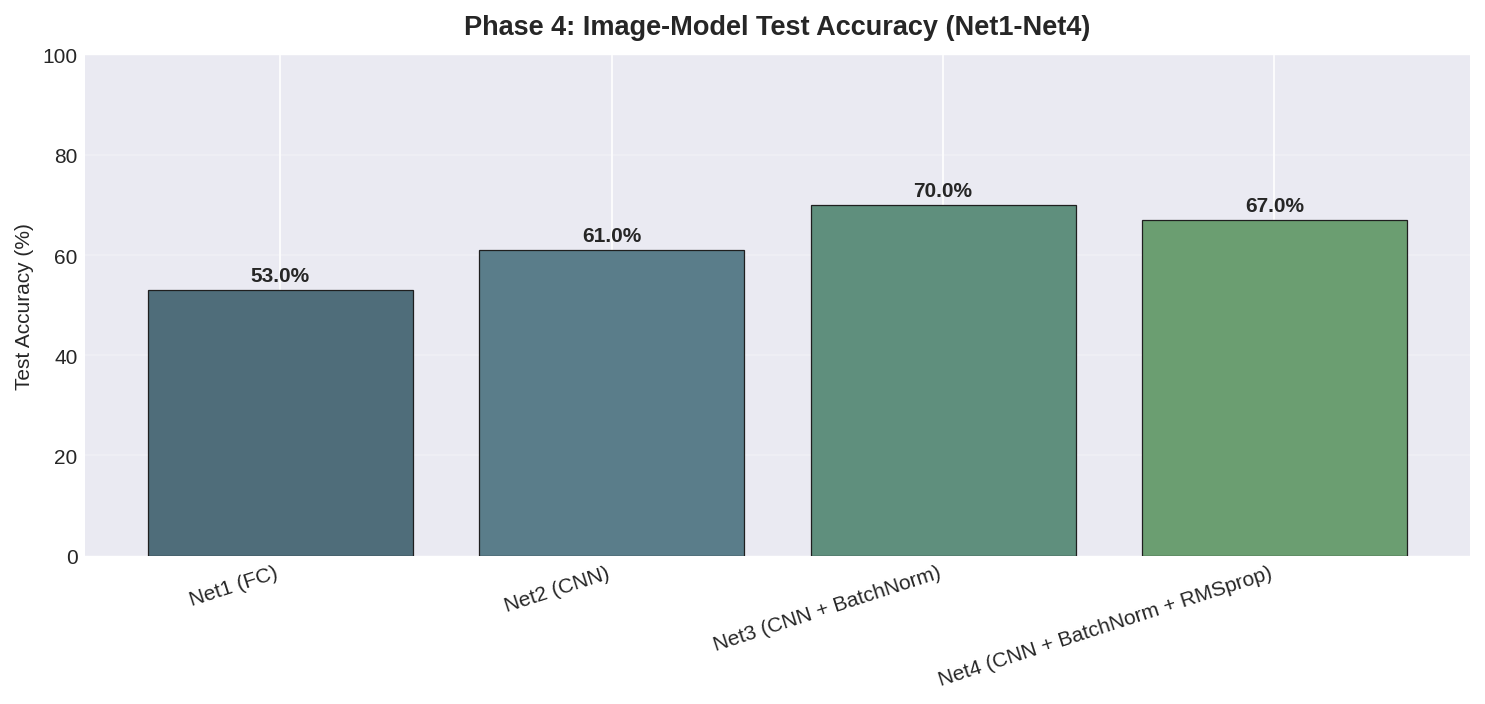
\includegraphics[width=\linewidth]{figures/comparison_image_models_phase4.png}
	\caption{Phase 4 image-model comparison (Net1--Net4).}
	\label{fig:image-phase4}
\end{figure}

\textbf{Net5 (LSTM), 69.0\%.} The sequence model on MFCC features performs strongly and is close to the best CNN result. This indicates that temporal evolution carries useful genre cues.

\textbf{Net6 (LSTM + GAN), 71.0\%.} Net6 is the best overall model and improves Net5 by \textbf{+2.0 points}. The gain is modest but consistent with useful augmentation from synthetic training samples.

\begin{figure}[t]
	\centering
	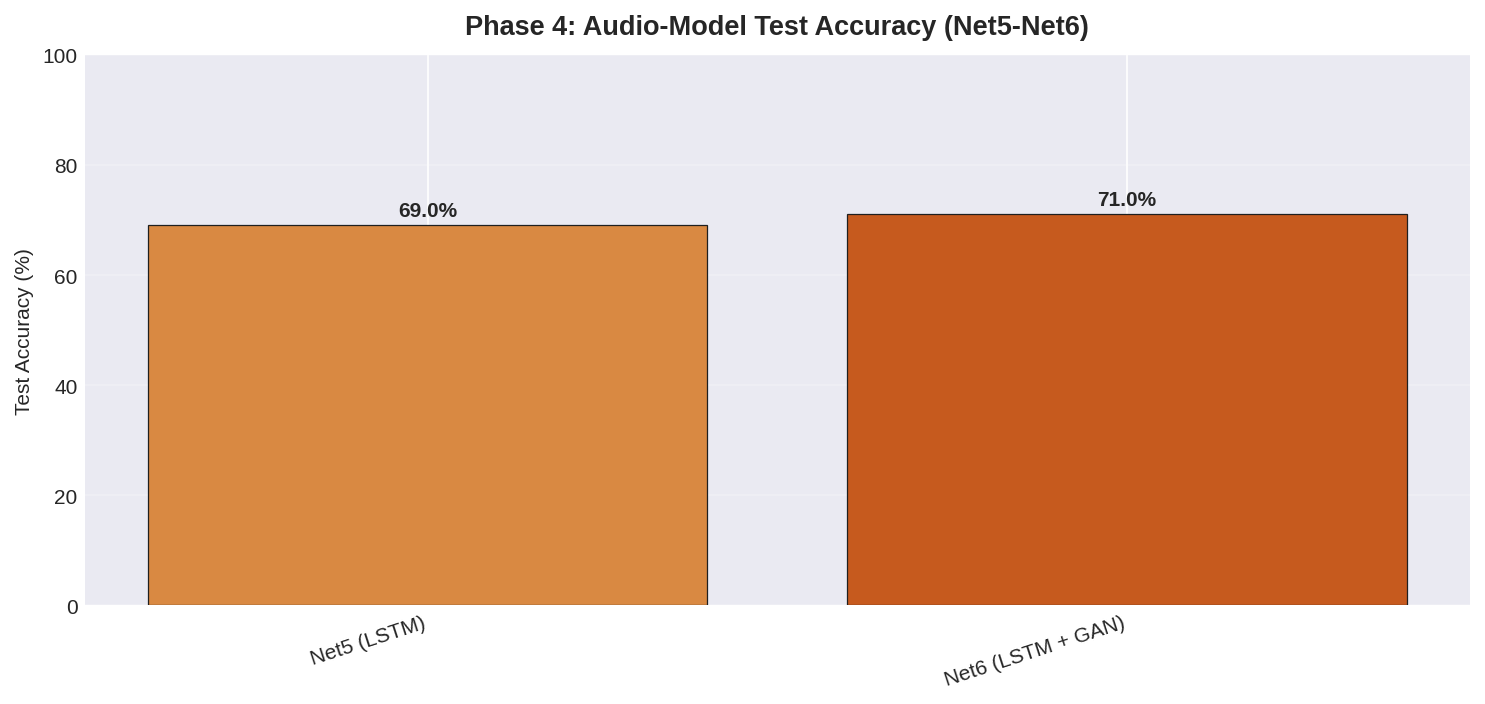
\includegraphics[width=\linewidth]{figures/comparison_audio_models_phase4.png}
	\caption{Phase 4 audio-model comparison (Net5--Net6).}
	\label{fig:audio-phase4}
\end{figure}

\begin{figure}[t]
	\centering
	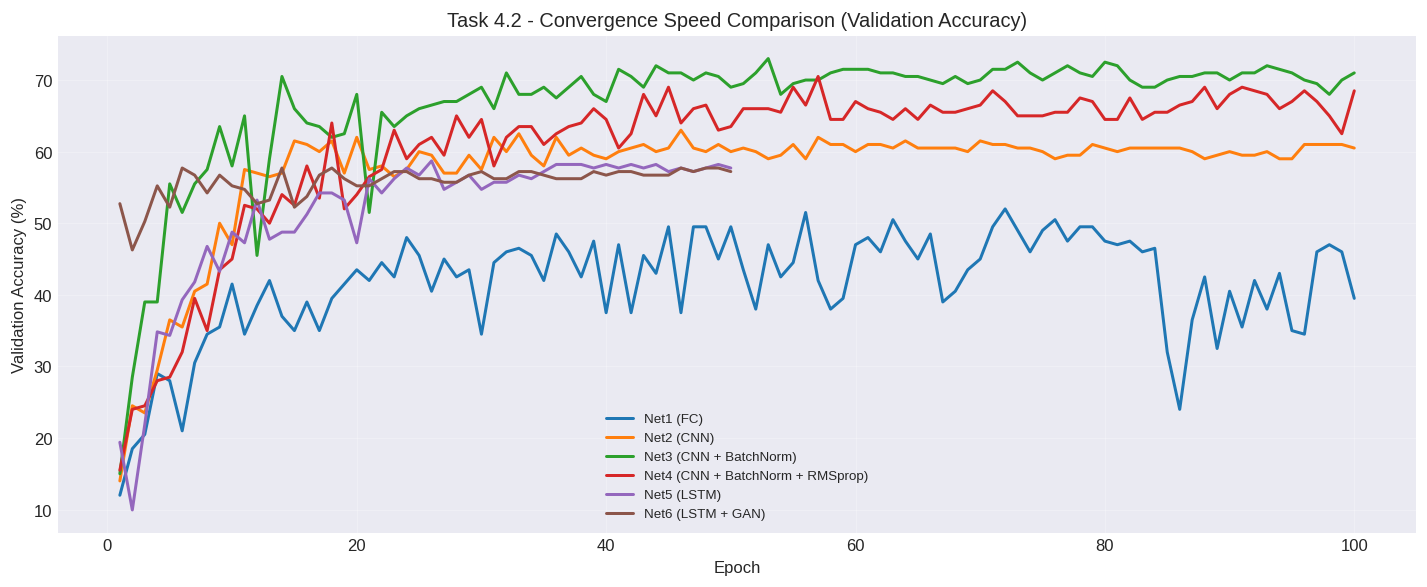
\includegraphics[width=\linewidth]{figures/phase4_convergence_speed.png}
	\caption{Phase 4 validation-accuracy convergence line graph (Task 4.2).}
	\label{fig:phase4-convergence}
\end{figure}

\subsection{Overall Discussion}

Figure~\ref{fig:all-phase4} summarizes the complete ranking across all six models. The top three models are Net6 (71.0\%), Net3 (70.0\%), and Net5 (69.0\%). Mean accuracy is \textbf{70.00\%} for audio models and \textbf{62.75\%} for image models, a \textbf{+7.25-point} advantage for the audio branch on this split.

\begin{figure}[t]
	\centering
	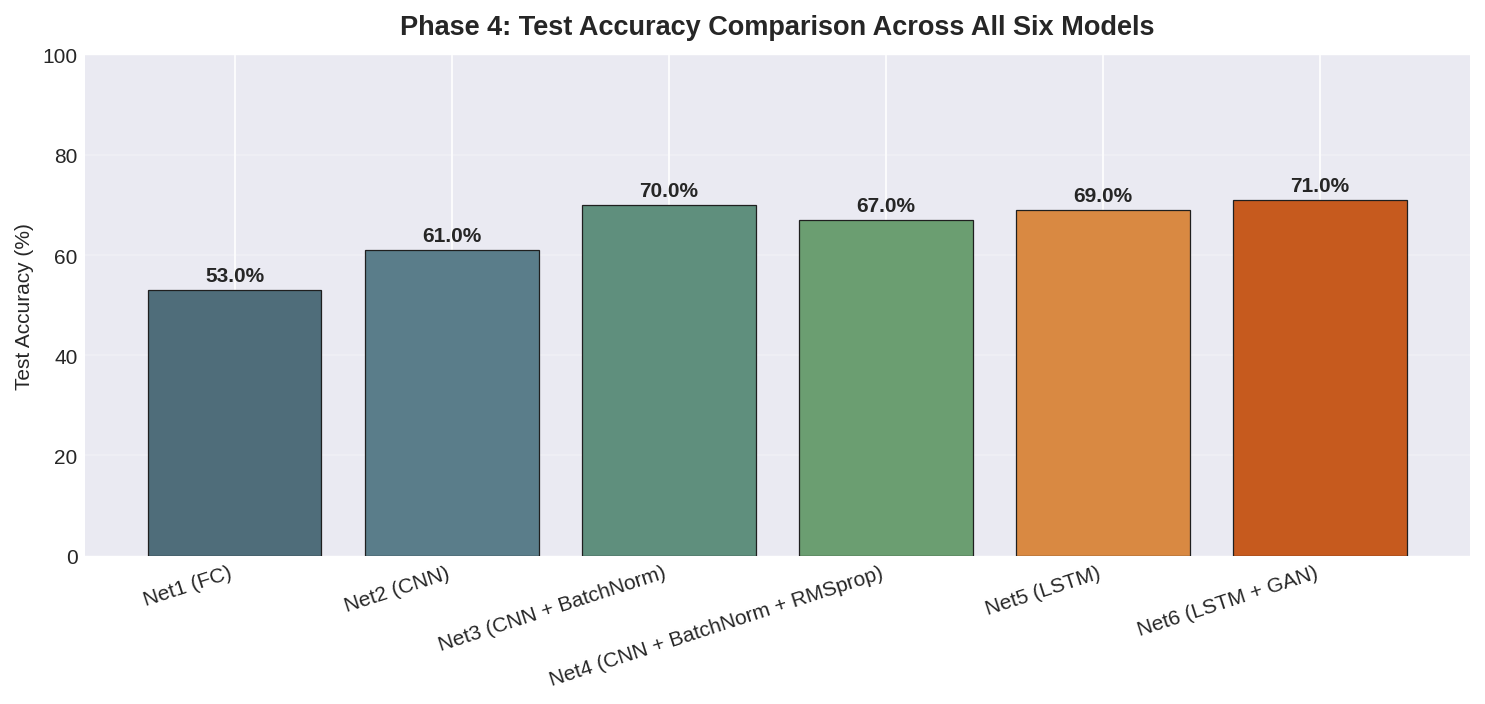
\includegraphics[width=\linewidth]{figures/comparison_all_models_phase4.png}
	\caption{Phase 4 test-accuracy comparison across all six models.}
	\label{fig:all-phase4}
\end{figure}

Genre-level analysis from Phase 4 shows \textbf{jazz} as the easiest class (mean recall 0.95) and \textbf{rock} as the hardest (mean recall 0.30). The most frequent aggregated confusion is \textbf{rock $\rightarrow$ country} (16 errors), which suggests overlap in rhythmic and timbral patterns for these genres in the current feature representation.

\begin{table}[t]
	\centering
	\caption{Complexity and training summary from \texttt{phase4\_model\_complexity.csv} and \texttt{phase4\_training\_time\_comparison.csv}.}
	\label{tab:phase4-complexity-time}
	\scriptsize
	\setlength{\tabcolsep}{3.5pt}
	\resizebox{\columnwidth}{!}{%
	\begin{tabular}{lccc}
		\toprule
		Model & Params (M) & Epoch@90\% Val & Train (s) \\
		\midrule
		N1 (FC) & 87.44 & 24 & 2.23 \\
		N2 (CNN) & 16.13 & 11 & 46.17 \\
		N3 (CNN+BN) & 66.63 & 14 & 63.74 \\
		N4 (CNN+BN+RMSp) & 66.63 & 18 & 63.45 \\
		N5 (LSTM) & 1.51 & 12 & 25.96 \\
		N6 (LSTM+GAN) & 1.51 & 1 & 44.26 \\
		\bottomrule
	\end{tabular}%
	}
\end{table}

\begin{table}[t]
	\centering
	\caption{Top confusion pairs from \texttt{phase4\_aggregated\_confusions.csv}.}
	\label{tab:phase4-top-confusions}
	\scriptsize
	\setlength{\tabcolsep}{3pt}
	\begin{tabular}{@{}lc@{}}
		\toprule
		Confusion Pair & Count \\
		\midrule
		rock $\rightarrow$ country & 16 \\
		blues $\rightarrow$ country & 6 \\
		hiphop $\rightarrow$ reggae & 6 \\
		blues $\rightarrow$ reggae & 6 \\
		metal $\rightarrow$ hiphop & 6 \\
		reggae $\rightarrow$ country & 4 \\
		\bottomrule
	\end{tabular}
\end{table}

\begin{table}[t]
	\centering
	\caption{Genre recall difficulty from \texttt{phase4\_genre\_recall\_difficulty.csv}.}
	\label{tab:phase4-genre-recall}
	\scriptsize
	\setlength{\tabcolsep}{3pt}
	\begin{tabular}{@{}lc@{}}
		\toprule
		Genre & Mean Recall \\
		\midrule
		jazz & 0.95 \\
		classical & 0.92 \\
		hiphop & 0.77 \\
		metal & 0.73 \\
		reggae & 0.63 \\
		disco & 0.63 \\
		pop & 0.60 \\
		blues & 0.50 \\
		country & 0.48 \\
		rock & 0.30 \\
		\bottomrule
	\end{tabular}
\end{table}